\documentclass[14pt]{beamer}
%\documentclass[handout,14pt]{beamer} %Makes Handouts
\usetheme{default} %Gray with fade at top
% \useoutertheme[subsection=false]{miniframes} %Supppress subsection in header
% \useinnertheme{rectangles} %Itemize/Enumerate boxes
% % \usecolortheme{seagull} %Color theme
% % \usecolortheme{rose} %Inner color theme

% \definecolor{light-gray}{gray}{0.75}
% \definecolor{dark-gray}{gray}{0.55}
% \setbeamercolor{item}{fg=light-gray}
% \setbeamercolor{enumerate item}{fg=dark-gray}

% \setbeamertemplate{navigation symbols}{}
% \setbeamertemplate{mini frames}{}
% %\setbeamercovered{dynamics}
% \setbeamerfont*{title}{size=\Large,series=\bfseries}
% \setbeamerfont{footnote}{size=\tiny}

% %\setbeameroption{notes on second screen} %Dual-Screen Notes
% %\setbeameroption{show only notes} %Notes Output

% \setbeamertemplate{frametitle}{\vspace{.5em}\bfseries\insertframetitle}
\newcommand{\heading}[1]{\noindent \textbf{#1}\\ \vspace{1em}}
\newcommand{\questions}{\frame{{\large Questions?}}}

\usepackage{bbding,color,multirow,times,ccaption,tabularx,graphicx,verbatim,booktabs}
\usepackage{colortbl} %Table overlays
\usepackage[english]{babel}
\usepackage[latin1]{inputenc}
\usepackage[T1]{fontenc}
\usepackage{lmodern}
\usepackage{alltt}

\usepackage{tikz}
\usetikzlibrary{shapes,arrows,decorations.pathreplacing,calc}



\usepackage{multirow}

% \setbeamertemplate{headline}
%  {%
%   \begin{beamercolorbox}{section in head/foot}
%   \insertsectionnavigationhorizontal{\textwidth}{}{}
%   \end{beamercolorbox}%
% }

\author[]{Santiago L\'opez Cariboni}
\institute{
  Universidad de la Rep\'ublica - dECON
}


\title{La implementaci\'on de experimentos de encuesta}

\date[]{}

\begin{document}

\frame{\titlepage}

\frame{\tableofcontents}

\frame{}

\section[Practical Issues]{Practical Issues}
\frame{\tableofcontents[currentsection,subsubsectionstyle=hide]}


\subsection{Participant Recruitment}
\frame{\tableofcontents[currentsection,currentsubsection,subsubsectionstyle=hide]}

\frame{

\frametitle{How do we find participants?}

\begin{itemize}\itemsep1em
\item Volunteers
	\begin{itemize}
	\item Volunteer Science
	\item In-house subject pool
	\end{itemize}

\item Paid crowdworkers
	\begin{itemize}
	\item Prolific Academic
	\item Mechanical Turk
	\item Crowdflower
	\end{itemize}

\item ``Representative'' samples
	\begin{itemize}
	\item Big players: YouGov, TNS, Gallup, Nielsen, GfK
	\item Others: Kantar, SSI, Lucid
	\end{itemize}
\end{itemize}

}

\frame{
\frametitle{SUTO Framework}
\begin{itemize}\itemsep0.5em
\item Cronbach (1986) talks about generalizability in terms of UTO
\item Shadish, Cook, and Campbell (2001) speak similarly of:
	\begin{itemize}
	\item \textbf{S}ettings
	\item \textbf{U}nits
	\item \textbf{T}reatments
	\item \textbf{O}utcomes
	\end{itemize}
\item External validity depends on all of these
\end{itemize}
}


\frame{
\begin{columns}[t]
\begin{column}{0.5\textwidth}
	\begin{block}{Population}
		\begin{itemize}
		\item Setting
		\item Units
		\item Treatments
		\item Outcomes
		\end{itemize}
	\end{block}
\end{column}
\begin{column}{0.5\textwidth}
	\begin{block}{Your Study}
		\begin{itemize}
		\item Setting
		\item Units
		\item Treatments
		\item Outcomes
		\end{itemize}
	\end{block}
\end{column}
\end{columns}

\vspace{0.5em}

\small

\only<2->{In your study, how do these correspond?\\}
\only<3->{\hspace{5.7em} how do these differ?\\}
\only<4->{\hspace{5.7em} do these differences matter?\\}

}

\frame{
\frametitle{Common Differences}
\begin{itemize}\itemsep1em
\item Most common thing to focus on is demographic representativeness
	\begin{itemize}
	\item Sears (1986): ``students aren't real people''
	\item \href{http://www.slate.com/articles/health_and_science/science/2013/05/weird_psychology_social_science_researchers_rely_too_much_on_western_college.html}{Western, educated, industrialized, rich, democratic (WEIRD) psychology participants}
	\end{itemize}
\item<2-> But do those characteristics actually matter?
\item<3-> Shadish, Cook, and Campbell tell us to think about:
	\begin{itemize}
	\item Surface similarities
	\item Ruling out irrelevancies
	\item Making discriminations
	\item Interpolation/extrapolation
	\end{itemize}
\end{itemize}
}

\frame{
\begin{center}
\includegraphics[height=\textheight]{./../images/coppock_et_al-1}
\end{center}
}

\frame{
\begin{center}
\includegraphics[height=\textheight]{./../images/coppock_et_al-2}
\end{center}
}

\questions

\subsection{Attention, Satisficing, and Noncompliance}
\frame{\tableofcontents[currentsection,currentsubsection,subsubsectionstyle=hide]}

\frame{

One final issue with unit-related sources of heterogeneity is how we handle or analyze survey-experimental data where we think participants misbehaved.

\vspace{1em}

\only<2->{This falls into a couple of broad categories:

\begin{itemize}
\item Noncompliance
\item Inattention
\item Survey Satisficing
\end{itemize}
}
}

\frame{

How should we deal with respondents that appear to not be paying attention, not ``taking'' the treatment, or not responding to outcome measures?

\begin{enumerate}
\item Keep them
\item Throw them away
\end{enumerate}

}

\frame{

\frametitle{Best Practice: Pre-Analysis Protocol}

\begin{itemize}\itemsep0.5em
\item Excluding respondents based on survey behavior is one of the easiest ways to ``p-hack'' an experimental dataset
	\begin{itemize}
	\item Inattention, satisficing, etc. will tend to reduce the size of the SATE
	\end{itemize}
\item So regardless of how you handle these respondents, these should be decisions that are made \textit{pre-analysis}
\end{itemize}

}


\frame[label=exclusion]{

\frametitle{{\normalsize When are you excluding participants?}}

    \begin{columns}[T]
    \begin{column}[T]{5cm}
        \begin{block}{\rule[-0.6ex]{0pt}{2.5ex}Pre-Treatment}
            \begin{itemize}\itemsep0.2em
                \item<2-> \hyperlink{satisficing}{Satisficing behaviors}
                \item<3-> Inattention
                \item<4-> Covariate-based selection
                \item<5-> Pretreated
            \end{itemize}
        \end{block}
    \end{column}
    \begin{column}[T]{5cm}
        \begin{block}{\rule[-0.6ex]{0pt}{2.5ex}Post-Treatment}
            \begin{itemize}\itemsep0.5em
                \item<6-> Speeding on treatment
                \item<7-> ``Failing'' a manipulation check
                \item<8-> Drop-off
            \end{itemize}
        \end{block}
    \end{column}
    \end{columns}

}


\frame{

\frametitle{Pre-Treatment Exclusion}

\begin{itemize}\itemsep0.5em
\item This is totally fine from a causal inference perspective
\item<2-> Advantages:
	\begin{itemize}
	\item Focused on engaged respondents
	\item Likely increase impact of treatment
	\end{itemize}
\item<3-> Disadvantages:
	\begin{itemize}
	\item Changing definition of sample (and thus population)
	\end{itemize}
\end{itemize}

}


\frame{

\frametitle{Post-Treatment Exclusion}

This is much more problematic because it involves controlling for a \textit{post-treatment} variable

}

\frame<1-3>[label=posttreatment]{

\begin{center}
\begin{tikzpicture}[>=latex',circ/.style={draw, shape=circle, node distance=5cm, line width=1.5pt}]
    \draw (0,0) node[left, text width=3cm, align=center] (X) {Information};
    \draw (5,0) node[right, text width=2cm, align=center] (Y) {Opinion};
    \draw<1-3>[->] (X) -- (Y);
    \draw[->] (4,-4) node[below, text width=3cm, align=center] (E) {Etc.} -- (Y);
	\draw<2-> (1,-2) node[text width=3cm, align=center] (M) {Manipulation Check};
	\draw<2-4>[->,thick,red] (X) -- (M);
    \draw<2-4>[->,thick,red] (M) -- (Y);
    \draw<3>[->] (E) -- (M);
\end{tikzpicture}
\end{center}

\small 
\only<2>{Risk that estimate of $\beta_1$ is diminished because effect is being carried through the manipulation check.}
\only<3>{Introduction of ``collider bias'' wherein values of the manipulation check are affected by other factors.}
}





\frame[label=posttreatment2]{

\frametitle{Post-Treatment Exclusion}

\small

\begin{itemize}\itemsep0.5em
\item Any post-treatment exclusion is problematic and should be avoided
\item<2-> Can estimate a LATE
	\begin{itemize}\footnotesize
	\item Interpretation: Effect of manipulation check among those whose value of the check can be changed by the treatment manipulation
	\end{itemize}
\item<3-> Non-response or attrition is the same as researcher-imposed exclusion
	\begin{itemize}\footnotesize
	\item Not problematic if MCAR
	\item Nothing really to be done if caused by treatment
	\end{itemize}
\end{itemize}

}

\againframe<3-4>{posttreatment}

\againframe<2->{posttreatment2}


\questions

\frame[label=satisficing]{
\frametitle{Apparent Satisficing}
\begin{itemize}\itemsep0.5em
\item Some common measures:
	\begin{itemize}
	\item ``Straightlining''
	\item Non-differentiation
	\item Acquiescence
	\item Nonresponse
	\item DK responding
	\item Speeding
	\end{itemize}
\item Difficult to detect and distinguish from ``real'' responses
\end{itemize}
}

\frame{
\frametitle{Metadata/Paradata}
\begin{itemize}\itemsep1em
\item<1-> Timing
	\begin{itemize}
	\item Some survey tools will allow you to time page
	\item Make a prior rules about dropping participants for speeding
	\end{itemize}
\item<2-> Mousetracking or eyetracking
	\begin{itemize}
	\item Mousetracking is unobtrusive
	\item Eyetracking requires participants opt-in
	\end{itemize}
\item<3-> Record focus/blur browser events
\end{itemize}
}

\frame{
\frametitle{Direct Measures}
\begin{itemize}\itemsep1em
\item How closely have you been paying attention to what the questions on this survey actually mean?
\item<2-> While taking this survey, did you engage in any of the following behaviors? Please check all that apply.
	\begin{itemize}
	\item Use your mobile phone
	\item Browse the internet
	\item \dots
	\end{itemize}
\end{itemize}
}



\frame{
\frametitle{{\normalsize Instructional Manipulation Check}}

\small

\only<2>{Do you agree or disagree with the decision to send British forces to fight ISIL in Syria? }We would like to know if you are reading the questions on this survey. If you are reading carefully, please ignore this question, do not select any answer below, and click ``next'' to proceed with the survey.\\

\vspace{0.5em}

\footnotesize
Strongly disagree\\
Somewhat disagree\\
Neither agree nor disagree\\
Somewhat agree\\
Strongly agree\\

\vspace{1em}
\only<2>{\hyperlink{exclusion}{\beamerbutton{Return}}}
}



\frame{

\frametitle{{\normalsize Treatment Noncompliance}}

\begin{itemize}\itemsep0.5em
\item Definition:\\{\small ``when subjects who were assigned to receive the treatment go untreated or when subjects assigned to the control group are treated'' \footnote{Gerber \& Green. 2012. \textit{Field Experiments}, p.132.}}
\item<2-> Several strategies
	\begin{itemize}
	\item ``As treated'' analysis
	\item ``Intention to treat'' analysis
	\item Estimate a LATE
	\end{itemize}
\end{itemize}

}

\frame{
\frametitle{{\normalsize Analyzing Noncompliance}}

\small

\begin{itemize}\itemsep0.5em
\item If noncompliance only occurs in one group, it is \textit{asymmetric} or \textit{one-sided}
\item We can ignore non-compliance and analyze the ``intention to treat'' effect, which will underestimate our effects because some people were not treated as assigned: $ITT = \overline{Y}_1 - \overline{Y}_0$
\item<2-> We can use ``instrumental variables'' to estimate the ``local average treatment effect'' (LATE) for those that complied with treatment: $LATE = \frac{ITT}{\% Compliant}$
\end{itemize}
}

\frame{
	\frametitle{{\large Local Average Treatment Effect}}
	\small
	\begin{itemize}\itemsep0.2em
	\item IV estimate is \textit{local} to the variation in $X$ that is due to variation in $D$
	\item This matters if effects are \textit{heterogeneous}
	\item LATE is effect for those who \textit{comply}
	\item Four subpopulations:
		\begin{itemize}\footnotesize
		\item Compliers: $X = 1$ only if $D = 1$
		\item Always-takers: $X = 1$ regardless of $D$
		\item Never-takers: $X = 0$ regardless of $D$
		\item Defiers: $X = 1$ only if $D = 0$
		\end{itemize}
	\item Exclusion restriction! Monotonicity!
	\end{itemize}
}



\questions




\subsection{Use of Covariates}
\frame{\tableofcontents[currentsection,currentsubsection,subsubsectionstyle=hide]}


\frame{

\frametitle{Discussion}

Consider the following:

\begin{itemize}
\item When \textbf{are we required to} include covariates in the analysis of an experiment?
\item When \textbf{are we allowed to} include covariates in the analysis of an experiment?
\item When \textbf{are we not allowed to} include covariates in the analysis of an experiment?
\end{itemize}

Discuss with a partner for 2 minutes.

}

\frame{

\begin{itemize}\itemsep1em
\item We never have to use covariates!
\item<2-> We may want to for:
	\begin{itemize}
	\item Subgroup comparisons
	\item Repeated/panel designs
	\item In case of noncompliance or attrition
	\end{itemize}
\item<3-> Any use of covariates should be planned!
\end{itemize}

}

\frame{

\frametitle{Block Randomization I}

{\small \textbf{Stratification:Sampling::Blocking:Experiments}}

\small

\begin{itemize}\itemsep0.5em
\item<2-> Basic idea: randomization occurs within strata defined before treatment assignment
\item<3-> CATE is estimate for each stratum; aggregated to SATE
\item<4-> Why?
	\begin{itemize}
	\item Eliminate chance imbalances
	\item Optimized for estimating CATEs
	\item More precise SATE estimate
	\end{itemize}
\end{itemize}

}

\begin{frame}[fragile]

\begin{center}
\begin{tabular}{lcccccccc}
Exp. & \multicolumn{4}{c}{Control} & \multicolumn{4}{c}{Treatment} \\ \midrule
1 & M & M & M & M & F & F & F & F \\
2 & M & M & M & F & M & F & F & F \\
3 & M & M & F & F & M & M & F & F \\
4 & M & F & F & F & M & M & M & F \\
5 & F & F & F & F & M & M & M & M \\ \bottomrule
\end{tabular}
\end{center}


{\scriptsize
\begin{verbatim}
# population of men and women
pop <- rep(c("Male", "Female"), each = 4)

# randomly assign into treatment and control
split(sample(pop, 8, FALSE), c(rep(0,4), rep(1,4)))
\end{verbatim}
}

\end{frame}

\frame{

\begin{center}

\begin{tabular}{rrrr}
Obs. & $X_{1i}$ & $X_{2i}$ & $D_i$ \\ \midrule
1 & Male & Old & 0 \\
2 & Male & Old & 1 \\  \midrule
3 & Male & Young & 1 \\
4 & Male & Young & 0 \\ \midrule
5 & Female & Old & 1 \\
6 & Female & Old & 0 \\ \midrule
7 & Female & Young & 0 \\
8 & Female & Young & 1 \\ \bottomrule
\end{tabular}
\end{center}

}

\frame[label=blocking2]{

\frametitle{Block Randomization II}

\begin{itemize}
\item Blocking ensures ignorability of all covariates used to construct the blocks
\item Incorporates covariates explicitly into the \textit{design}
\item<2-> When is blocking \textit{statistically} useful?
	\begin{itemize}
	\item<3-> If those covariates affect values of potential outcomes, blocking reduces the variance of the SATE
	\item<4-> Most valuable in small samples
	\item<5-> Not valuable if all blocks have similar potential outcomes
	\end{itemize}
\end{itemize}

}



\frame{

\frametitle{Statistical Properties I}

\small

Complete randomization:\\
$$SATE = \frac{1}{n_1}\sum Y_{1i} - \frac{1}{n_0}\sum Y_{0i}$$

\vspace{2em}

Block randomization:\\
$$SATE_{blocked} = \sum_{1}^{J} \left( \dfrac{n_j}{n} \right)  (\widehat{CATE}_j)$$

}


\frame{

\begin{center}

\begin{tabular}{rrrrrr}
Obs. & $X_{1i}$ & $X_{2i}$ & $D_i$ & $Y_i$ & CATE \\ \midrule
1 & Male & Old & 0 & 5 & \multirow{2}{*}{\onslide<2->{5}} \\
2 & Male & Old & 1 & 10 \\  \midrule
3 & Male & Young & 1 & 4 & \multirow{2}{*}{\onslide<3->{3}} \\
4 & Male & Young & 0 & 1 \\ \midrule
5 & Female & Old & 1 & 6 & \multirow{2}{*}{\onslide<4->{4}} \\
6 & Female & Old & 0 & 2 \\ \midrule
7 & Female & Young & 0 & 6 & \multirow{2}{*}{\onslide<5->{3}} \\
8 & Female & Young & 1 & 9 \\ \bottomrule
\end{tabular}
\end{center}

}

\frame{

\frametitle{SATE Estimation}

\begin{align*}
SATE &= \left(\dfrac{2}{8}*5\right) + \left(\dfrac{2}{8}*3\right) + \left(\dfrac{2}{8}*4\right) + \left(\dfrac{2}{8}*3\right) \\ \vspace{1em}
&= 3.75
\end{align*}

\onslide<2->{The blocked and unblocked estimates are the same here because $Pr(Treatment)$ is constant across blocks and blocks are all the same size.}

}

\frame{

\frametitle{SATE Estimation}

\small

\begin{itemize}
\item We can use weighted regression to estimate this in an OLS framework
\item Weights are the inverse prob. of being treated w/in block
\begin{itemize}
\item Pr(Treated) by block: $p_{ij} = Pr(D_i = 1 | J=j) $
\item Weight (Treated): $ w_{ij} = \dfrac{1}{p_{ij}} $
\item Weight (Control): $ w_{ij} = \dfrac{1}{1-p_{ij}} $
\end{itemize}
\end{itemize}

}


\frame{

\frametitle{Statistical Properties II}

\small

Complete randomization:\\
$$\widehat{SE}_{SATE} = \sqrt{\dfrac{\widehat{Var}(Y_0)}{n_0} + \dfrac{\widehat{Var}(Y_1)}{n_1}}$$

\vspace{1em}

Block randomization:\\
$$\widehat{SE}_{SATE_{blocked}} = \sqrt{\sum_{1}^{J} \left( \dfrac{n_j}{n} \right)^2  \widehat{Var}{(SATE_j)}}$$

\only<2->{When is the blocked design more efficient?}

}


\frame{

\frametitle{Practicalities}

\begin{itemize}\itemsep1em
\item Blocked randomization only works in exactly the same situations where stratified sampling works
	\begin{itemize}
	\item Need to observe covariates pre-treatment in order to block on them
	\item Work best in a panel context
	\end{itemize}
\item In a single cross-sectional design that might be challenging
	\begin{itemize}
	\item Some software can block ``on the fly''
	\end{itemize}
\end{itemize}

}

\questions


\subsection{Effect Heterogeneity}
\frame{\tableofcontents[currentsection,currentsubsection,subsubsectionstyle=hide]}

\frame{
\frametitle{{\large Detecting Effect Heterogeneity}}

Always block if you expect heterogeneity!

\begin{itemize}\itemsep0.5em
\item QQ-plots: Suggestive evidence
\item Regression using treatment-by-covariate interactions
\item<2-> (Replication and meta-analysis)
\end{itemize}

}



\frame{

\frametitle{Suggestive Evidence}

We can never know $Var(TE_i)$! \onslide<2->{But\dots}

\begin{itemize}\itemsep0.5em
\item<2-> Quantile-quantile plots
	\begin{itemize}
	\item<3-> Compare the distribution of $Y_0$'s to distribution of $Y_1$'s
	\item<3-> If homogeneity, a vertical shift in $Y_1$'s
	\item<3-> If heterogeneity, a slope $\neq$ 1
	\end{itemize}
\item<4-> Equality of variance tests
	\begin{itemize}
	\item<4-> If homogeneity, variance should be equal
	\item<4-> If heterogeneity, variances should differ
	\end{itemize}
\end{itemize}

}

\begin{frame}[fragile]

\frametitle{QQ Plots}

{\scriptsize
\begin{verbatim}
# y_0 data
set.seed(1)
n <- 200
y0 <- rnorm(n) + rnorm(n, 0.2)

# y_1 data (homogeneous effects)
y1a <- y0 + 2 + rnorm(n, 0.2)
# y_1 data (heterogeneous effects)
y1b <- y0 + rep(0:1, each = n/2) + rnorm(n, 0.2)

qqplot(y0, y1a, pch=19, xlim=c(-3,5), ylim=c(-3,5), asp=1)
curve((x), add = TRUE)
qqplot(y0, y1b, pch=19, xlim=c(-3,5), ylim=c(-3,5), asp=1)
curve((x), add = TRUE)
\end{verbatim}

}

\end{frame}


\frame{

\begin{center}
\only<1>{\includegraphics[height=\textheight]{./../images/qqplot1}}
\only<2>{\includegraphics[height=\textheight]{./../images/qqplot2}}
\end{center}

}

\begin{frame}[fragile]

\frametitle{Equality of Variance tests}

\footnotesize

\begin{verbatim}
> var.test(y0, y1a)

        F test to compare two variances

data:  y0 and y1a
F = 0.60121, num df = 199, denom df = 199, 
  p-value = 0.0003635
alternative hypothesis: 
  true ratio of variances is not equal to 1
95 percent confidence interval:
 0.4549900 0.7944289
sample estimates:
ratio of variances 
         0.6012131 
\end{verbatim}

\end{frame}

\begin{frame}[fragile]

\frametitle{Equality of Variance tests}

\footnotesize

\begin{verbatim}
> var.test(y0, y1b)

        F test to compare two variances

data:  y0 and y1b
F = 0.53483, num df = 199, denom df = 199,
  p-value = 1.224e-05
alternative hypothesis:
  true ratio of variances is not equal to 1
95 percent confidence interval:
 0.4047531 0.7067133
sample estimates:
ratio of variances 
         0.5348312
\end{verbatim}

\end{frame}


\questions


\frame{\frametitle{Regression Estimation}}

\frame{

\frametitle{{\normalsize Aside: Regression Adjustment in Experiments, Generally}}

\begin{itemize}\itemsep0.5em
\item Recall the general advice that we do not need covariates in the regression to ``control'' for omitted variables (because there are none)
\item Including covariates can reduce variance of our SATE by explaining more of the variation in $Y$
\end{itemize}

}

\frame{

\frametitle{Scenario}

Imagine two regression models. Which is correct?

\begin{enumerate}
\item Mean-difference estimate of SATE is ``not significant''
\item Regression estimate of SATE, controlling for sex, age, and education, is ``significant''
\end{enumerate}

\onslide<2->{This is a small-sample dynamic, so make these decisions pre-analysis!}

}

\frame{

\frametitle{{\normalsize Treatment-Covariate Interactions}}

\normalsize

\begin{itemize}
\item The regression paradigm allows us to estimate CATEs using interaction terms
	\begin{itemize}
	\item $X$ is an indicator for treatment
	\item $M$ is an indicator for possible moderator
	\end{itemize}
\item<2-> SATE: $Y = \beta_0 + \beta_1 X + e$
\item<3-> CATEs: $$Y = \beta_0 + \beta_1 X + \beta_2 M + \beta_3 X*M + e$$
	\begin{itemize}
	\item<4-> Homogeneity: $\beta_3 = 0$
	\item<4-> Heterogeneity: $\beta_3 \neq 0$
	\end{itemize}

\end{itemize}

}


\questions

\section[Quiz]{Handling ``Broken'' Experiments}
\frame{\tableofcontents[currentsection]}

\frame{

\Large

\begin{center}
Quiz time!
\end{center}

}


\frame{
\frametitle{Compliance}

\large

\begin{enumerate}\itemsep0.5em
\item<1-> What is compliance?
\item<2-> How can we analyze experimental data when there is noncompliance?
\end{enumerate}
}

\frame{
\frametitle{Balance testing}

\normalsize

\begin{enumerate}\itemsep0.5em
\item<1-> What does randomization ensure about the composition of treatment groups?
\item<2-> What can we do if we find a covariate imbalance between groups?
\item<3-> How can we avoid this problem entirely?
\end{enumerate}
}


\frame{
\frametitle{Nonresponse and Attrition}

\large

\begin{enumerate}\itemsep0.5em
\item<1-> Do we care about outcome nonresponse in experiments?
\item<2-> How can we analyze experimental data when there is outcome nonresponse or post-treatment attrition?
\end{enumerate}
}


\frame{
\frametitle{Manipulation checks}

\large

\begin{enumerate}\itemsep0.5em
\item<1-> What is a manipulation check? What can we do with it?
\item<2-> What do we do if some respondents ``fail'' a manipulation check?
\end{enumerate}
}



\frame{
\frametitle{Null effects}

\large

\begin{enumerate}\itemsep0.5em
\item<1-> What should we do if we find our estimated $\widehat{SATE} = 0$?
\item<2-> What does it mean for an experiment to be \textit{underpowered}?
\item<3-> What can we do to reduce the probability of obtaining an (unwanted) ``null effect''?
\end{enumerate}
}


\frame{
\frametitle{Effect heterogeneity}

\large

\begin{enumerate}\itemsep0.5em
\item<1-> What should we do if, post-hoc, we find evidence of effect heterogeneity?
\item<2-> What can we do pre-implementation to address possible heterogeneity?
\end{enumerate}
}


\frame{
\frametitle{Representativeness}

\large

\begin{enumerate}\itemsep0.5em
\item<1-> Under what conditions is a design-based, probability sample necessary for experimental inference?
\item<2-> What kind of causal inferences can we draw from an experiment on a descriptively unrepresentative sample?
\end{enumerate}
}

\frame{
\frametitle{Peer Review}

\large

\begin{enumerate}\itemsep0.5em
\item<1-> What should we do if a peer reviewer asks us to ``control'' for covariates in the analysis?
\item<2-> What should we do if a peer reviewer asks us to include or exclude particular respondents from the analysis?
\end{enumerate}
}


\questions



\section{Research Ethics}
\frame{\tableofcontents[currentsection]}

\frame{
\frametitle{History: Key Moments}

\small

\begin{enumerate}
\item Tuskegee (1932-1972) and Guatemala (1946-1948) Studies
\item Nuremberg Code (1947)
\item Helsinki Declaration (1964)
\item U.S. 45 CFR 46 (1974) and ``Common Rule'' (1991)
\item The Belmont Report (1979)
\item EU Data Protection Directive (1995; 2012)
	\begin{itemize}
	\item UK Data Protection Act (1998)
	\end{itemize}
\end{enumerate}
}


\frame{
	\frametitle{Helsinki Declaration}
	
	\small
	\begin{itemize}
	\item Adopted by the World Medical Association in 1964\footnote{\url{http://www.bmj.com/content/2/5402/177}}
	\item Narrowly focused on medical research
	\item Expanded the Nuremberg Code
		\begin{itemize}
		\item Relaxed consent requirements
		\item Risks should not exceed benefits
		\item Institutionalization of ethics oversight
		\end{itemize}
	\item<2-> Do these rules apply to non-medical research?
	\end{itemize}

}

\frame{
	\frametitle{The Belmont Report}
	
	\small
	\begin{itemize}
	\item Commissioned by the U.S. Government in 1979\footnote{\url{http://www.hhs.gov/ohrp/humansubjects/guidance/belmont.html}}
	\item Three overarching principles:
		\begin{enumerate}
		\item Respect for persons
		\item Beneficence
		\item Justice
		\end{enumerate}
	\item Three policy implications:
		\begin{itemize}
		\item Informed consent
		\item Assessment of risks/benefits
		\item Care for vulnerable populations
		\end{itemize}
	\end{itemize}

}

\frame{
\frametitle{Benefits and Harm}
	\begin{itemize}\itemsep1em
	\item What is a ``benefit''?
	\item What is a ``harm''?
	\item How do we balance the two?
	\end{itemize}
}


\frame{

\frametitle{Ethical Considerations}

\begin{itemize}
\item Most ethical issues are not unique to \textit{experimental} social science
\item Some especially important issues:
	\begin{enumerate}
	\item Randomization
	\item Informed consent
	\item Privacy
	\item Deception
	\item Publication bias
	\end{enumerate}
\end{itemize}

}

\frame{

\frametitle{I. Randomization}

\begin{itemize}
\item Is it ethical to randomize?
\end{itemize}

}



\frame{
	\frametitle{II. Informed Consent}
	\begin{itemize}
	\item Persons must consent to being a research subject
	\item<2-> What this means in practice is complicated
		\begin{itemize}
		\item What is consent?
		\item What is ``informed'' consent?
		\item What exactly do they have to consent to?
		\end{itemize}
	\item<3-> Cross-national variations
		\begin{itemize}
		\item Consent forms required in U.S.
		\item Not required in UK
		\end{itemize}
	\end{itemize}

}


\frame{
	\frametitle{III. Privacy}
	\begin{itemize}\itemsep0.5em
	\item Under EU Data Protection Directive (1995), data can be processed when:
		\begin{itemize}
		\item Consent is given
		\item Data are used for a ``legitimate'' purpose
		\item Anonymous or confidential
		\end{itemize}
	\item These rules have become more expansive under GDPR (in force as of 2018)
	\item Data cannot leave the EU except under conditions
	\end{itemize}

}

\frame{
	\frametitle{III. Privacy}
	\begin{itemize}\itemsep1em
	\item Experimental might be additionally sensitive
	\item<2-> Answers reflect ``manipulated'' attitudes, behaviors, perceptions, etc. that respondents may not have given in another setting
	\end{itemize}

}



\frame{

\frametitle{IV. Deception}

\begin{itemize}
\item Major distinction between psychology tradition and economics tradition\footnote{Dickson, E. 2011. ``Economics versus Psychology Experiments.'' \textit{Cambridge Handbook of Experimental Political Science}.}
	\begin{itemize}
	\item Purpose of the study
	\item Purpose of specific items or tasks
	\item Order or length of questionnaire
	\end{itemize}
\item<2-> Psychologists focus on \textit{debriefing}
\item<3-> Within economics, norms about \textit{acts of omission} versus \textit{acts of commission}
	\begin{itemize}
	\item<4-> Omission: In a multi-round trust game, an additional round is added
	\item<5-> Commission: Telling respondents it is a dictator game, but it is actually a trust game
	\end{itemize}
\end{itemize}


}


\frame{

\frametitle{V. Publication Bias}

\begin{itemize}\itemsep0.5em
\item Publication bias not typically discussed as an ethical question
\item<2-> If studies are meant to policy or practical implications, then we care about PATE or a set of CATEs, including whether their effects are positive, negative, or zero.
\item<3-> Publication bias (toward ``significant'' results) invites wasting resources on treatments that actually don't work
\end{itemize}

}



\frame{
	\frametitle{{\normalsize Lots of Other Ethical Questions}}
	\begin{enumerate}
	\item<2-> Funding
	\item<3-> Independence and Politicization
	\item<4-> Vulnerable populations (e.g. children, sick)
	\item<5-> Incentives
	\item<6-> Cross-national research
	\item<7-> End uses/users of research
	\item<8-> Others\dots
	\end{enumerate}
}

\questions

\section{Conclusion}
\frame{\tableofcontents[currentsection]}

\frame{

\frametitle{Learning Outcomes}

\small

By the end of the week, you should be able to\dots

\begin{enumerate}
\item<2-> Explain how to analyze experiments quantitatively.
\item<3-> Explain how to design experiments that speak to relevant research questions and theories.
\item<4-> Evaluate the uses and limitations of several common survey experimental paradigms.
\item<5-> Identify practical issues that arise in the implementation of experiments and evaluate how to anticipate and respond to them.
\end{enumerate}

}


\frame{
	\frametitle{Wrap-up}
	\begin{itemize}
	\item Thanks to all of you!
	\item Stay in touch (\href{mailto:t.leeper@lse.ac.uk}{t.leeper@lse.ac.uk})
	\item Good luck with your research!
	\end{itemize}
}












\appendix


\section[More Designs]{Beyond One-Shot Designs}
\frame{\tableofcontents[currentsubsection,subsubsectionstyle=hide]}

\frame{

\frametitle{{\normalsize Beyond One-shot Designs}}


\begin{itemize}\itemsep0.5em
\item Surveys can be used as a measurement instrument for a field treatment or a manipulation applied in a different survey panel wave
	\begin{enumerate}
	\item Measure effect duration in two-wave panel
	\item Solicit pre-treatment outcome measures in a two-wave panel
	\item Measure effects of field treatment in post-test only design
	\item Randomly encourage field treatment in pre-test and measure effects in post-test
	\end{enumerate}
\item<2-> Problems? Compliance \& nonresponse
\end{itemize}

}

\frame{

\frametitle{{\normalsize I. Effect Duration}}

\begin{itemize}\itemsep0.5em
\item Use a two- (or more-) wave panel to measure duration of effects
	\begin{itemize}
	\item T1: Treatment and outcome measurement
	\item T2+: Outcome measurement
	\end{itemize}
\item Two main concerns
	\begin{itemize}
	\item Attrition
	\item Panel conditioning
	\end{itemize}
\end{itemize}

}

\frame{

\frametitle{{\normalsize II. Within-Subjects Designs}}

\small

\begin{itemize}
\item Estimate treatment effects as a difference-in-differences
\item Instead of using the post-treatment mean-difference in $Y$ to estimate the causal effect, use the difference in pre-post differences for the two groups:
	\begin{align*}
	(\hat{Y}_{0,t+1} - \hat{Y}_{0,t}) - (\hat{Y}_{j,t+1} - \hat{Y}_{j,t})
	\end{align*}
\item<2-> Advantageous because variance for paired samples decreases as correlation between $t_0$ and $t_1$ observations increases
\end{itemize}

}


\frame{
	\begin{center}
	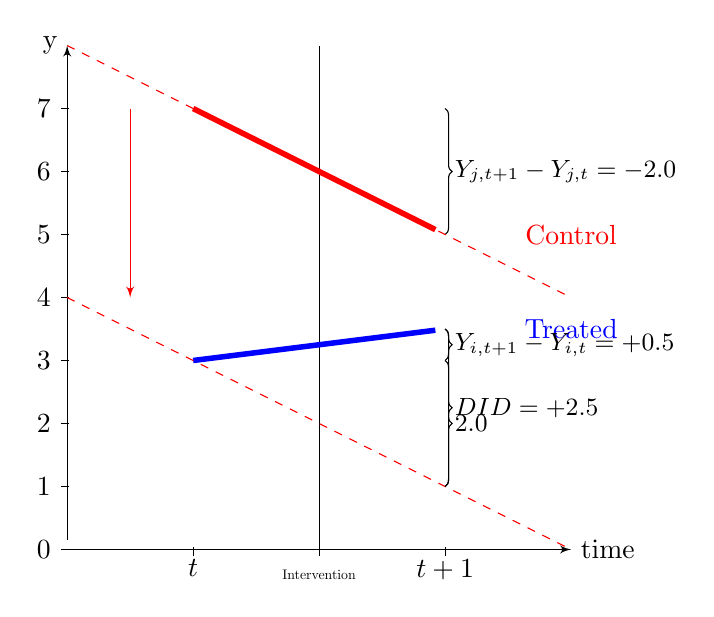
\begin{tikzpicture}[>=latex', scale=0.8]
        \draw[->] (0,0) node (origin) {}  -- (8,0) node[right] (xaxis) {time};
        \draw[->] (origin) -- (0,8) node[left] (yaxis) {y};
        % x ticks
        \foreach \x in {2,4,6}
        	\draw (\x,1pt) -- (\x,-3pt) node[anchor=north] {};
        \draw (2,0) node[below] (before) {$t$};
        \draw (6,0) node[below] (after) {$t+1$};
        \draw (4,-0.25) node[below, scale=0.5] (IV) {Intervention};
        % y ticks
        \foreach \y in {0,...,7}
             \draw (1pt,\y) -- (-3pt,\y) node[anchor=east] {$\y$};
        % intervention
        \draw (4,0) -- (4,8);

        % line
        \draw<2-> (6,3.5) node (tr) {};
        \draw<3-> (6,5) node (ctrl) {};
        \draw<2-3>[blue] (8,3.5) node (trlab) {Treated};
        \draw<3-3>[red] (8,5) node (ctrllab) {Control};        
        \draw<2->[blue, line width=2pt] (2,3) -- (tr);
        \draw<3->[red, line width=2pt] (2,7) -- (ctrl);
        
        % diffs
        \draw<4-6>[right,decorate,decoration={brace,mirror}] 
        	(6,3) -- (6,3.5) node[right, pos=0.5] (idiff) {\small $Y_{i,t+1} - Y_{i,t} = +0.5$};
        \draw<4-6>[right,decorate,decoration={brace}] 
            (6,7) -- (6,5) node[right, pos=0.5] (jdiff) {\small $Y_{j,t+1} - Y_{j,t} = -2.0$};
        
        % trends
        \draw<5-6>[red,->] (1,7) -- (1,4);
        \draw<5->[red, dashed] (0,8) -- (8,4);
        \draw<5->[red, dashed] (0,4) -- (8,0);
        \draw<6>[right,decorate,decoration={brace}] 
            (6,3) -- (6,1) node[right, pos=0.5] (idiff2) {\small $2.0$};
        \draw<7>[right,decorate,decoration={brace}] 
            (6,3.5) -- (6,1) node[right, pos=0.5] (idiff2) {\small $DID = +2.5$};
                        
        
    \end{tikzpicture}
    \end{center}
}


\frame{

	\frametitle{{\normalsize Threats to Validity}}
	
	\small
	
	As soon as time comes into play, we have to worry about threats to validity.\footnote{Shadish, Cook, and Campbell (2002)}
	
	\begin{enumerate}
	\item<2-> History (simultaneous cause)
	\item<3-> Maturation (time trends)
	\item<4-> Testing (observation changes respondents)
	\item<5-> Instrumentation (changing operationalization)
	\item<6-> Instability (measurement error)
	\item<7-> Attrition
	\end{enumerate}
}






\frame{

\frametitle{{\normalsize III. Randomized Field Treatment}}

\small

\begin{itemize}\itemsep-0.2em
\item Examples:
	\begin{enumerate}
	\item<2-> Citizens randomly sent a letter by post encouraging them to reduce water usage
	\item<3-> Different local media markets randomly assigned to receive different advertising
	\end{enumerate}
\item<4-> Survey is used to measure outcomes, when treatment assignment is already known
\item<5-> Issues
	\begin{itemize}
	\item<6-> Nonresponse
	\item<6-> Noncompliance
	\end{itemize}
\end{itemize}

}

\frame{
\frametitle{Noncompliance}

\small

\begin{itemize}
\item Compliance is when individuals receive and accept the treatment to which they are assigned
\item Noncompliance:\\{\small ``when subjects who were assigned to receive the treatment go untreated or when subjects assigned to the control group are treated'' \footnote{Gerber \& Green. 2012. \textit{Field Experiments}, p.132.}}
\item This causes problems for our analysis because factors other than randomization explain why individuals receive their treatment
\item Lots of methods for dealing with this, but the consequence is generally reduced power
\end{itemize}
}

\frame{
\frametitle{Asymmetric Noncompliance}

\small

\begin{itemize}\itemsep0.25em
\item Noncompliance \textit{asymmetric} if only in one group
\item We can ignore non-compliance and analyze the ``intention to treat'' effect, which will underestimate our effects because some people were not treated as assigned\\
	$ITT = \overline{Y}_1 - \overline{Y}_0$
\item We can use ``instrumental variables'' to estimate the ``local average treatment effect'' (LATE) for those that complied with treatment:\\
	$LATE = \frac{ITT}{Percent Compliant}$
\item We can ignore randomization and analyze data ``as-treated'', but this makes our study no longer an experiment
\end{itemize}
}

\frame{
	\frametitle{{\large Local Average Treatment Effect}}
	\small
	\begin{itemize}\itemsep0.2em
	\item IV estimate is \textit{local} to the variation in $X$ that is due to variation in $D$
	\item LATE is effect for those who \textit{comply}
	\item Four subpopulations:
		\begin{itemize}\footnotesize
		\item Compliers: $X = 1$ only if $D = 1$
		\item Always-takers: $X = 1$ regardless of $D$
		\item Never-takers: $X = 0$ regardless of $D$
		\item Defiers: $X = 1$ only if $D = 0$
		\end{itemize}
	\item Exclusion restriction! Monotonicity!
	\end{itemize}
}

\frame{
\frametitle{Two-Sided Noncompliance}
\begin{itemize}\itemsep1em
\item Two-sided noncompliance is more complex analytically
\item Stronger assumptions are required to analyze it and we won't discus them here
\item Best to try to develop a better design to avoid this rather than try to deal with the complexities of analyzing a broken design
\end{itemize}
}





\frame{

\frametitle{{\normalsize IV. Treatment Encouragement}}

\small

\begin{itemize}\itemsep-0.2em
\item Design:
	\begin{itemize}
	\item T1: Encourage treatment
	\item T2: Measure effects
	\end{itemize}
\item Examples:
	\begin{enumerate}
	\item Albertson and Lawrence\footnote{Albertson \& Lawrence. 2009. ``After the Credits Roll.'' \textit{American Politics Research} 37(2): 275--300. \href{http://doi.org/10.1177/1532673X08328600}{10.1177/1532673X08328600}.}
	\end{enumerate}
\item<2-> Issues
	\begin{itemize}
	\item<3-> Nonresponse
	\item<3-> Noncompliance
	\end{itemize}
\end{itemize}

}


\frame{

\frametitle{{\normalsize Treatment Noncompliance}}

\begin{itemize}\itemsep0.5em
\item<2-> Several strategies
	\begin{itemize}
	\item ``As treated'' analysis
	\item ``Intention to treat'' analysis
	\item Estimate a LATE
	\end{itemize}
\end{itemize}

}

\questions







\section{Behavioral Outcomes}

\frame{

\frametitle{Heterogeneity due to \textit{O}utcomes}

\begin{itemize}\itemsep1em
\item This is expected!
	\begin{itemize}
	\item E.g., non-equivalent outcomes
	\end{itemize}
\item Reasonable to explore multiple outcomes
	\begin{itemize}
	\item Multiple comparisons
	\item Power considerations
	\item Construct validity
	\end{itemize}
\item<2-> What outcomes you measure depend on your theory
\item<3-> Lots of potential for behavioral measures!
\end{itemize}

}


\frame{
\frametitle{Behavioural measures}
Some behaviours that can be directly measured through survey questionnaires.

\vspace{1em}

\only<2->{Three broad categories:}
\begin{enumerate}
\item<3-> Behavioural measures that provide survey paradata % (response latency, reading times, answer switching, nonresponse)
\item<4-> Behavioural measures that operationalize attitudes % IAT
\item<5-> Behavioural measures that operationalize behaviours % (e.g., political participation; purchasing)
\end{enumerate}
}


\frame{
\frametitle{Behavioural Measures for Paradata}

Why?
	\begin{itemize}
	\item Respondents use of the survey tells us something meaningful about their behaviour
	\end{itemize}
\only<2->{What?
	\begin{itemize}
	\item<3-> Nonresponse
	\item<4-> Response latencies
	\item<5-> Reading times
	\item<6-> Answer switching
	\item<7-> Eye tracking
	\item<8-> Mouse tracking
	\item<9-> Smartphone metadata
	\end{itemize}
}
}


\frame{
\frametitle{Behavioural Measures for Attitudes}

Why?
	\begin{itemize}
	\item Attitudinal self-reports might be ``cheap talk''
	\end{itemize}

\vspace{1em}
\only<2->{What?
	\begin{itemize}
	\item<3-> Implicit Association Test
	\item<4-> Incentivized Survey questions
	\end{itemize}
}
}



\frame{

\frametitle{Behavioural Measures for Behaviour}

Why?
	\begin{itemize}
	\item We want to observe or affect behaviour (e.g., in an experiment)
	\end{itemize}
	
\vspace{1em}
\only<2->{What? 
	\begin{itemize}
	\item Directly measure or initiate a direct measure of a behaviour
	\item May be measured by something that occurs within the confines of the survey or something outside of the survey
	\end{itemize}
}
}


\frame<1-2>[label=infochoice]{

\frametitle{Example 1:\\Active Information Choice}

\begin{itemize}\itemsep0.5em
\item<2-> ``Followed link'' identification\footnote{Guess, AM. 2015. ``Measure for Measure.'' \textit{Political Analysis} 23: 59--75. \href{http://doi.org/10.1093/pan/mpu010}{doi:10.1093/pan/mpu010} }

\item<3-> Information boards\footnote{Leeper, TJ. 2014. ``The Informational Basis for Mass Polarization.'' \textit{Public Opinion Quarterly} 78(1): 27--46. \href{http://doi.org/10.1093/poq/nft045}{doi:10.1093/poq/nft045}}

\item<4-> Video choice\footnote{Arceneaux, K \& Johnson, M. 2012. \textit{Changing Minds or Changign Channels}. Chicago: The University of Chicago Press.}

\item<5-> Dynamic Process Tracing Environment \footnote{\url{https://dpte.polisci.uiowa.edu/dpte/}}
\end{itemize}

}

\frame{\includegraphics[width=\textwidth]{./../images/linksguess.png}}

\againframe<2-3>{infochoice}

\frame{\includegraphics[width=\textwidth]{./../images/leeper.png}}

\againframe<3-5>{infochoice}

\frame{\includegraphics[width=\textwidth]{./../images/dpte1.png}}
\frame{\includegraphics[width=\textwidth]{./../images/dpte2.png}}
\frame{\includegraphics[width=\textwidth]{./../images/dpte3.png}}



\frame{

\frametitle{Example 2:\\Sign-up/Enrolment}

An extension of information choice behaviour would be explicit engagement in other kinds of (small) behaviours, such as:

\begin{itemize}\itemsep0.5em
\item Entering an email address to receive information or join a mailing list \footnote{Leeper, TJ. 2017. ``How Does Treatment Self-Selection Affect Inferences About Political Communication?'' \textit{Journal of Experimental Political Science}: In press.} \footnote{Bolsen, Druckman, \& Cook. 2014. ``Communication and Collective Actions.'' \textit{Journal of Experimental Political Science} 1(1): 24--38. \href{http://doi.org/10.1017/xps.2014.2}{doi:10.1017/xps.2014.2}}

\item Signing up for an appointment or further interaction
\end{itemize}

}


\frame<1>[label=incentivised]{
\frametitle{Example 3:\\Incentivised Survey Questions}

Definitions:

\begin{itemize}\itemsep0.5em
\item A survey question is just a self-report
\item An \textit{incentivized} survey question attached financial gains or losses to the answer options
\end{itemize}

\vspace{1em}
\only<2->{
Paradigm could be applied to any measure of behavioural intentions to avoid cheap talk.
}

}

\frame{

\includegraphics[width=\textwidth]{./../images/eckelgrossman.png}

\vspace{2em}
{\tiny Eckel \& Grossman. 2008 ``Forecasting risk attitudes.'' \textit{Journal of Economic Behavior \& Organization} 68(1): 1--17. \href{http://doi.org/10.1016/j.jebo.2008.04.006}{doi:10.1016/j.jebo.2008.04.006}\par }
}

\againframe<1->{incentivised}


\frame[label=purchasing]{
\frametitle{Example 4:\\Purchasing Decisions}

Common ways to study purchasing behaviour include:

\begin{itemize}
\item<2-> Direct attitudinal questions
\item<3-> Retrospective and prospective self-reports
\item<4-> Conjoint experiments
\end{itemize}

\only<5->{Another way is embedding a purchase in a survey.\footnote{Bolsen, T. 2011. ``A Lightbulb Goes On.'' \textit{Political Behavior} 35(1): 1--20.  \href{http://doi.org/10.1007/s11109-011-9186-5}{10.1007/s11109-011-9186-5}
}}

}

\frame{

\begin{center}
\includegraphics[width=.45\textwidth]{./../images/lightbulb1.png}
\includegraphics[width=.38\textwidth]{./../images/lightbulb2.png}
\end{center}

\vspace{1em}

{\tiny 
Source: Wikimedia Commons (\href{https://commons.wikimedia.org/wiki/File:06_Spiral_CFL_Bulb_2010-03-08_(white_back).jpg}{Sun Ladder}, \href{https://commons.wikimedia.org/wiki/File:Gluehlampe_01_KMJ.jpg}{KMJ}) \par }

}


\frame{

\frametitle{Example 5:\\Donations}

\begin{itemize}\itemsep1em
\item Miller and Krosnick\footnote{Miller, Krosnick, \& Lowe. N.d. ``The Impact of Policy Change Threat on Financial Contributions to Interest Groups.'' Working paper.} asked for charitable donations via cheque directly as part of a paper-and-pencil survey

\item<2-> Klar and Piston\footnote{Klar \& Piston. 2015. ``The influence of competing organisational appeals on individual donations.'' \textit{Journal of Public Policy} 35(2): 171--91. \href{http://doi.org/10.1017/S0143814X15000203}{doi:10.1017/S0143814X15000203}} offered respondents a survey incentive up-front for participation and then later offered them a chance to donate (a portion of payment) to a charity
\end{itemize}

}




\frame{

\frametitle{Example 6:\\Web Tracking Data}

\begin{enumerate}\itemsep1em
\item Active installation of a tracking app, such as YouGov Pulse\footnote{\url{https://yougov.co.uk/find-solutions/profiles/pulse/}} \footnote{Guess, AM. N.d. ``Media Choice and Moderation.'' Working paper, \url{https://dl.dropboxusercontent.com/u/663930/GuessJMP.pdf}.}

\item Post-hoc collection of web history files using something like Web Historian \footnote{\url{http://www.webhistorian.org/}}
\end{enumerate}
}



\frame<1-2>[label=other]{
\frametitle{Other Possibilities}

\begin{itemize}\itemsep1em
\item<2-> Coordination tasks
	\begin{itemize}
	\item Synchronous group tasks\footnote{Mao, Mason, Suri, Watts. 2016. ``An Experimental Study of Team Size and Performance on a Complex Task.'' \textit{PLoS ONE} 11(4): e0153048. \href{http://doi.org/10.1371/journal.pone.0153048}{doi:10.1371/journal.pone.0153048}} 
	\item Game play
	\item Simulations
	\end{itemize}
\item<3-> Offering incentives to perform future behaviour (tracked elsewhere)
\item<4-> OAuth/API integrations w/ other platforms
	\begin{itemize}
	\item Merging website usage data w/ survey data
	\item Treating website sign-up or usage as behavioural outcomes
	\item Linking with smartphone metadata
	\end{itemize}
\end{itemize}
}

\frame{\includegraphics[width=\textwidth]{./../images/mao.png}}


\againframe<2->{other}


\frame{}

\frame{

\frametitle{Some principles for survey measures of behaviour}

\begin{enumerate}\itemsep1em
\item<2-> Know why you are collecting a behavioural measure!
\item<3-> Know whether you are studying a past, present, or future behaviour.
\item<4-> Be creative! Recognise possibilities and limitations of any given survey mode.
\item<5-> Validate, validate, validate!
\end{enumerate}

}

\frame{

\frametitle{Activity!}

\large 

\begin{center}
With a partner, brainstorm how one or more these behavioural measures might be applied to a survey experiment (either as outcome, treatment, covariate, or behavioural check) relevant to your own work or your organisation.
\end{center}

}



\end{document}
